%%%%%%%%%%%%%%%%%%%%%%%%%%%%%%%%%%%%%%%%%%%%%%%%%%%%%%%%%%
%%
%% MARK: Title
%%
%%%%%%%%%%%%%%%%%%%%%%%%%%%%%%%%%%%%%%%%%%%%%%%%%%%%%%%%%%

\chapter*{\S B13. Cotangent Space of the Half-Line}
\setcounter{footnote}{0}


\begin{abstract}
  We investigate the nature and structure of the cotangent space of the embedded half-line
  $\Delta = \LeftClosedInterval{0,\infty}\,\subset \RR$.
\end{abstract}

%%%%%%%%%%%%%%%%%%%%%%%%%%%%%%%%%%%%%%%%%%%%%%%%%%%%%%%%%%
%%
%% MARK: Exercise 1
%%
%%%%%%%%%%%%%%%%%%%%%%%%%%%%%%%%%%%%%%%%%%%%%%%%%%%%%%%%%%

Consider the half-line $\Delta = \LeftClosedInterval{0,\infty}\,\subset \RR$,
equipped with the subset diffeology.
We have seen above, in ``$1$-Forms on Half-Lines'',
that every $1$-form $\alpha$ on $\Delta$ is the pullback of some $1$-form on $\RR$.
In other words, there exists a smooth function $a \in \Cinfty(\RR,\RR)$ such that
$$
  \alpha(P)_r(\delta r) = a(P(r)){\partial P(r) \over \partial r}\delta r,
  $$
where $P$ is a plot in $\Delta$, $r\in \Domain(P)$ and $\delta r$ is a vector in $\RR^n$,
with $n$ the dimension of the plot $P$.
One can also write
$$
  \alpha(P)_r(\delta r) = a(x)\delta x,
  $$
with $P : r \mapsto x$ and $\delta x = D(P)_r(\delta r)$.
We have also seen that the value of $\alpha$ at any point $x\neq 0$ is given by $a(x)$,
and that the value of $\alpha$ at $0$ is $0$.
Therefore, the map
$$
  \pi : \Delta \times \DForms^1(\Delta) \to \RR \times \RR,
  \quad \mbox{defined by} \quad
  \pi(x,\alpha) = (x, x a(x)),
  $$
gives a representation of the cotangent space $T^*(\Delta)$ \cite[6.48]{PIZ13},
where its image is equipped with the pushforward diffeology.
Indeed,
if $\pi(x,\alpha) = \pi(x',\alpha')$,
then $x=x'$ and if $x\neq 0$, then $a(x)=a(x')$.
If $x=0$,
then for any $\alpha$ and $\alpha'$,
$\pi(0,\alpha)= (0,0) = \pi(0,\alpha')$.
Since every $1$-form vanishes at the origin,
$(0,0)=\pi(0,\alpha)$ represents the value of $\alpha$ at $x=0$,
for all $\alpha$.

It is now time to investigate the diffeology on the set
$$
  \Val(\pi) = \{(0,0)\} \cup \OpenInterval{0,\infty} \times \RR
  $$
when it is equipped with the pushforward diffeology by $\pi$.

\begin{Article}{Real functions vanishing at the origin.}{}
  Let $f \in \Cinfty(\RR,\RR)$ such that $f(0)=0$.
  Then,
  there exists $\varphi \in \Cinfty(\RR,\RR)$ such that $f(x)=x\varphi(x)$,
  for all $x \in \RR$.
  
  Let $\Cinfty_0(\RR,\RR)$ be the subset of real smooth functions vanishing at the origin,
  equipped with the induced diffeology of the functional diffeology on $\Cinfty(\RR,\RR)$.
  Then, the map
  $$
    j : \Cinfty_0(\RR,\RR) \to \Cinfty(\RR,\RR)
    \quad \mbox{defined by} \quad
    j(f) = \varphi : x \mapsto {f(x) \over x}
    $$
  is a diffeomorphism.
\end{Article}

\begin{proof}
  First of all,
  if $x\neq 0$, $\varphi(x) = f(x)/x$.
  For $x=0$, $\varphi$ is extended by continuity and $\varphi(0)=f'(0)$.
  Next,
  it is clear that the map $j : f\mapsto \varphi$ is bijective.
  Now let us consider a plot $r \mapsto f_r$ in $\Cinfty_0(\RR,\RR)$.
  Applying Taylor's formula with remainder \cite[\textsection\,8.14.3]{Die70a},
  we obtain,
  since $f_r(0)=0$ for all $r$:
  $$
    f_r(x) = x f_r'(0) + x^2\int_0^1(1-t) f''_r(xt)\, dt.
    $$
  Since $\varphi_r(x) = f_r(x)/x$, we get
  $$
    \varphi_r(x) = f_r'(0) + x\int_0^1(1-t) f''_r(xt)\, dt.
    $$
  This expression shows clearly,
  for $f$ constant in $r$,
  that $\varphi$ is smooth.
  It shows,
  moreover,
  that $(r,x) \mapsto \varphi_r(x)$ is smooth,
  that is,
  $r \mapsto \varphi_r$ is a plot of $\Cinfty(\RR,\RR)$.
  Conversely,
  if $r \mapsto \varphi_r$ is a plot,
  then $r \mapsto [x \mapsto x\varphi_r(x)]$ is obviously a plot.
  Therefore,
  $j$ is a diffeomorphism.
\end{proof}

\begin{Article}{Representing $T^*(\Delta)$.}{}
  Let us factorize the projection $\pi : (x,\alpha) \to (x, x a(x))$ by
  $$
    (x,\alpha) \mapsto (x, f=[x\mapsto x a(x)]) \mapsto (x, f(x)=(x, x a(x))).
    $$
  Thanks to the previous article,
  the first arrow $(x,\alpha) \mapsto (x, f=[x\mapsto x a(x)])$ is a diffeomorphism from $\Delta \times \DForms^1(\Delta)$ to $\Delta \times \Cinfty_0(\Delta,\RR)$.
  The second arrow
  $$
    \Eval: (x,f) \mapsto (x,f(x)),
    $$
  defined on $\Delta \times \Cinfty_0(\Delta,\RR)$, is an \textit{evaluation map}.
  
  \smallskip\noindent 1) The cotangent space $T^*(\Delta)$ is diffeomorphic to $\{(0,0)\} \cup \OpenInterval{0,\infty} \times \RR$,
  equipped with the pushforward diffeology by $\Eval$.
  
  \smallskip\noindent 2) This diffeology,
  on $\{(0,0)\} \cup \OpenInterval{0,\infty} \times \RR$,
  is not the subset diffeology of $\RR^2$;
  it is strictly finer.
\end{Article}

\begin{figure}
  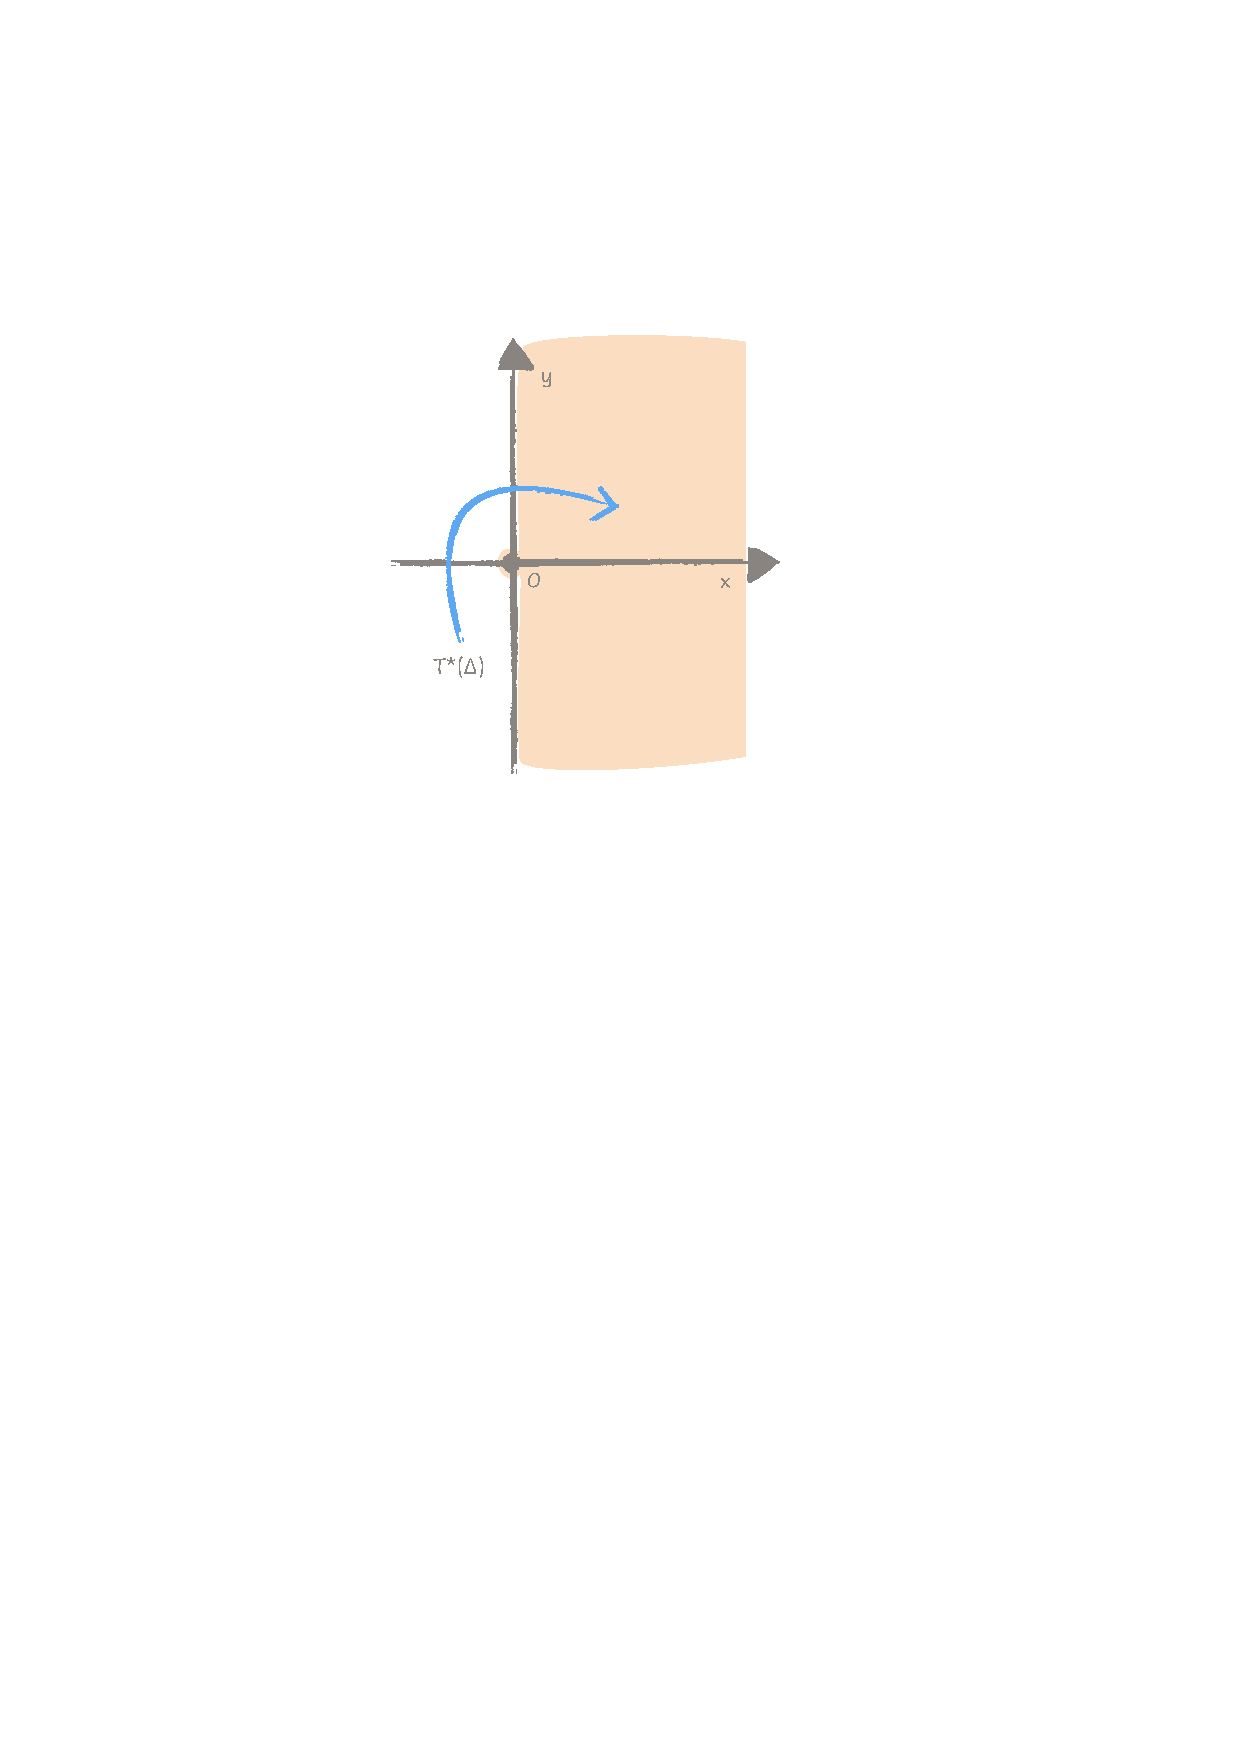
\includegraphics[width=.45\textwidth]{Figures/Cotangent-HL.pdf}
  \vspace{-.5\baselineskip}
  \caption{The representation of $T^*(\Delta)$.}
\end{figure}

\begin{proof}
  Indeed,
  consider the $1$-plot $\gamma : t\mapsto (x(t)=t^2,\, y(t)=t)$ of $\{(0,0)\} \cup \OpenInterval{0,\infty} \times \RR$ for the subset diffeology.
  Assume that there exists a local lift of $\gamma$ in $\Delta \times \Cinfty_0(\Delta,\RR)$ near $0$,
  that is,
  a smooth path $t \mapsto f_t$ in $\Cinfty_0(\RR,\RR)$ such that $y(t) = f_t(x(t))$.
  According to Article 1,
  there exists a smooth path $t \mapsto a_t$ such that $f_t(x)=x a_t(x)$.
  Thus,
  $y(t)=x(t)a_t(x(t))$,
  that is,
  $t = t^2 a_t(t^2)$,
  i.e. $a_t(t^2)=1/t$.
  But this is impossible since $t\mapsto a_t(t^2)$ is defined at $t=0$ (and moreover smooth).
  Therefore, $\Eval$ is not a subduction onto $\{(0,0)\} \cup \OpenInterval{0,\infty} \times \RR$ when this set is equipped with the subset diffeology.
  In other words,
  not all plots of the subset diffeology are plots for the cotangent diffeology.
  The cotangent diffeology is then finer than the subset diffeology.
\end{proof}
